\documentclass[20pt,landscape,dvips]{foils} 
% add 'draft' option above to exclude image when compiling
\usepackage[french]{babel}
\usepackage[utf8]{inputenc}  
\usepackage{csquotes} 
%\MakeOuterQuote{"}
\frenchspacing
\DecimalMathComma

\usepackage{latexsym}
\usepackage{amsmath,amssymb,amsfonts}
\usepackage{MnSymbol}
\usepackage{url}
\usepackage{graphicx}
%\usepackage[dvipsnames]{xcolor}
\usepackage{hyperref}
\usepackage{alltt}
\usepackage{pifont,manfnt}
\usepackage[dvipsnames,table]{xcolor}
\usepackage{subfig}
%\usepackage{enumerate}
%\usepackage{colortbl}
\usepackage{multirow,hhline}
\usepackage{cclicenses}
\setlength\parindent{0pt}
\hypersetup{colorlinks=true,citecolor=black,urlcolor=black,linkcolor=black}
\usepackage[style=verbose]{biblatex}
\bibliography{refs}

\newcommand{\highlight}[1]{\textcolor{Plum}{\bfseries #1}}
\newcommand{\remark}[1]{%
%\centerline{
\begin{center}
\framebox[.9\textwidth][t]{
\ding{46} 
\parbox[t]{.8\textwidth}{\small #1}}
\end{center}}

\DeclareMathOperator*{\inlaw}{\sim}
\newcommand{\iid}{\inlaw_{\text{i.i.d.}}}
%\newcommand{\iid}{\mathop{\mathrm{diag}}}
\newcommand{\pobs}{p_{\text{obs}}}

\reversemarginpar
\def\mark{\marginpar{\dbend}}

%\newcommand{\bm}[1]{\mbox{\boldmath{$#1$}}}
\renewcommand{\abstractname}{Summary}
\newcommand\bs{\char '134}   %  a backslash character for the \tt font
%\renewcommand\refname{Additional Readings}

% customize header/footer
\rightheader{}
% Note about the copyleft symbol:
% I use a custom reversed and circled "c" char because \textcopyleft in
% the textcomp package does not support sans serif font.
% Also, "c" is shifted horizontally by 1ex to align with the circle.
%\Restriction{\mbox{\raisebox{1.5ex}{\rotatebox{180}{\textcircled{c\kern.1ex}}} 2009}, \url{www.aliquote.org}}
% now I use the CC licence...
% \Restriction{\cc 2016 \VCRevision}
\Restriction{\cc 2016 Module 11 EESPE}

\title{Méthodes psychométriques en qualité de vie}
\author{Christophe Lalanne\\EA 7334 REMES\\ Unité de Méthodologie des critères d’évaluation\\Université Paris-Diderot, Sorbonne Paris-Cité\\}
\date{
\includegraphics[height=18ex]{logo.eps}}

%%% This file has been generated by the vc bundle for TeX.
%%% Do not edit this file!
%%%
%%% Define Git specific macros.
\gdef\GITHash{f4328f7906d309e9224e3e5c2f7f36477f44e69f}%
\gdef\GITAbrHash{f4328f7}%
\gdef\GITParentHashes{136657e4877819e72dc9ebb2f209631a2a8d1057}%
\gdef\GITAbrParentHashes{136657e}%
\gdef\GITAuthorName{Christophe Lalanne}%
\gdef\GITAuthorEmail{ch.lalanne@gmail.com}%
\gdef\GITAuthorDate{2016-07-06 10:29:58 +0200}%
\gdef\GITCommitterName{Christophe Lalanne}%
\gdef\GITCommitterEmail{ch.lalanne@gmail.com}%
\gdef\GITCommitterDate{2016-07-06 10:29:58 +0200}%
%%% Define generic version control macros.
\gdef\VCRevision{\GITAbrHash}%
\gdef\VCAuthor{\GITAuthorName}%
\gdef\VCDateRAW{2016-07-06}%
\gdef\VCDateISO{2016-07-06}%
\gdef\VCDateTEX{2016/07/06}%
\gdef\VCTime{10:29:58 +0200}%
\gdef\VCModifiedText{\textcolor{red}{with local modifications!}}%
%%% Assume clean working copy.
\gdef\VCModified{0}%
\gdef\VCRevisionMod{\VCRevision}%


\begin{document}
\LogoOff
\maketitle
\rightfooter{\quad\textsf{\thepage}}



%---------------------------------------------------------------Slide-
\foilhead{Outline}
\begin{itemize}
\item Définition des mesures subjectives en santé, intérêt et enjeu.
\item Approche psychométrique de la mesure.
\item Propriétés d'un bon instrument de mesure.
\item Modèles de mesure.
\item Exemple dans le domaine de la qualité de vie.
\end{itemize}


%---------------------------------------------------------------Slide-
\foilhead{Les mesures subjectives en santé}

Mesure subjective recueillie chez le patient

Patient reported outcome


%---------------------------------------------------------------Slide-
\foilhead{}

\bigskip
{\centering 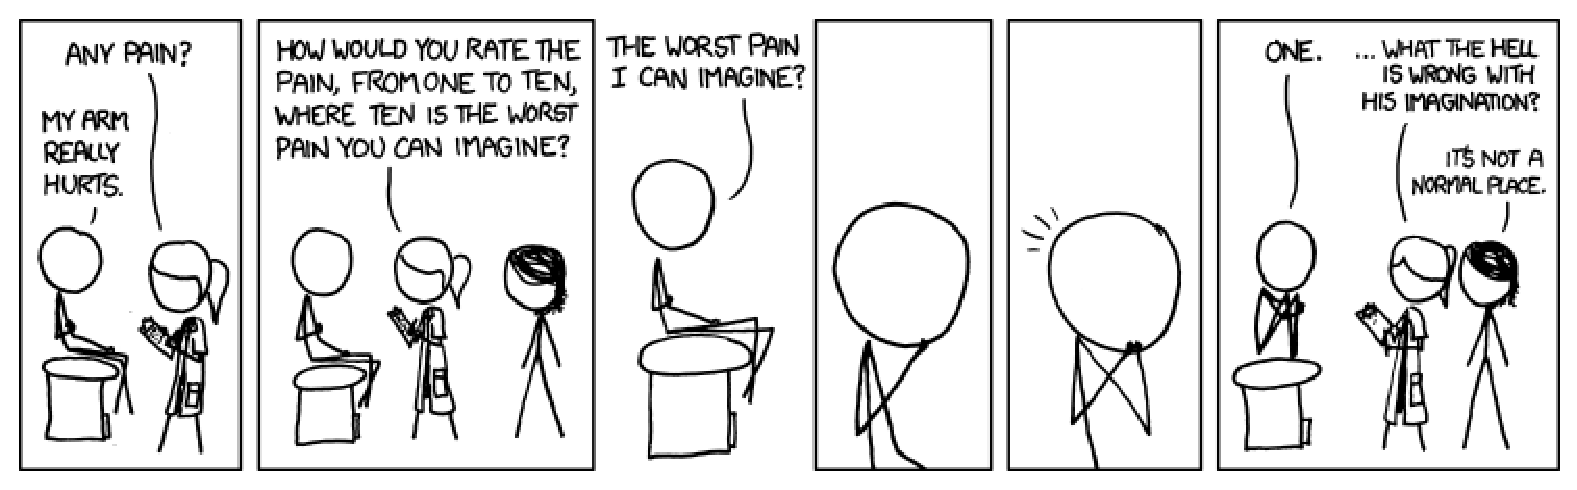
\includegraphics[width=\textwidth]{figs/pain.eps}\par}

%---------------------------------------------------------------Slide-
\foilhead{Instruments et mesures}

Un instrument est utilisé pour mettre en relation ou associer
\textcolor{Apricot}{quelque chose observé dans le monde réel} à
\textcolor{CornflowerBlue}{quelque chose de mesurable dans un certain cadre
  conceptuel}.

On parlera de \textcolor{Apricot}{variable manifeste} (p.ex., réponse à la
question "vous sentez-vous déprimé le matin en vous réveillant") et de
\textcolor{CornflowerBlue}{variable latente} (p.ex., "état dépressif" du
patient). 

On peut voir le processus de mesure comme une tâche consistant à assigner des
nombres à des catégories, ou réciproquement\autocite{Stevens1946,DeBoeck2005}.

%---------------------------------------------------------------Slide-
\foilhead{Construction d'un instrument de mesure\autocite{Wilson2005}}

\begin{itemize}
\item A \highlight{Construct map} features a coherent and substantive
  definition for the content of the construct which is composed of an
  underlying continuum (for ordering respondents and/or items
  responses).
\item \highlight{Items design} deals with the standardized
  construction of items that are supposed to stimulate responses,
  assimilable to observations about the construct. 
\item The \highlight{Outcome space} is the set of well-defined
  categories, finite and exhaustive, ordered, context-specific, and
  research-based.
\item A \highlight{Measurement model} is needed in order to relate the
  scored outcomes from the items design and the outcome space back to
  the construct that was the original inspiration of the items.
\end{itemize}

%---------------------------------------------------------------Slide-
\foilhead{Modèles à variables latentes}

La nature des variables manifestes et latentes permet généralement de guider le
choix d'un modèle statistique
\autocites{Bartholomew2011,RabeHesketh2008}.

\begin{center}\small
  \begin{tabular}{|c|c|c|c|}
    \cline{3-4}
    \multicolumn{2}{c|}{}&\multicolumn{2}{c|}{\textcolor{Apricot}{Variables manifestes}} \\
    \cline{3-4}
    \multicolumn{2}{c|}{}&\multicolumn{1}{c|}{Métrique} & \multicolumn{1}{c|}{Catégorielle} \\
    \hline
    \multirow{2}{*}{\textcolor{CornflowerBlue}{Variables latentes}} & Métrique & \highlight{Analyse factorielle} & \highlight{Analyse en traits latents} \\
    \cline{2-4}
    & Catégorielle & Analyse en profils latents & Analyse en classe latente\\
\hline
  \end{tabular}
\end{center}


%---------------------------------------------------------------Slide-
\foilhead{Illustration}

301 enfants de deux écoles auxquels on a administré 26 tests permettant d'évaluer les compétences suivantes : \textcolor{CornflowerBlue}{spatiales}, verbales, vitesse de raisonnement, mémoire, mathématiques.

\begin{quotation}
  Holzinger, K. J. and Swineford, F. A. \emph{A study in factor analysis: The stability
  of a bi-factor solution}. Supplementary Education Monographs, 48. University of
  Chicago, 1939.  
\end{quotation}

%---------------------------------------------------------------Slide-
\foilhead{Illustration}

{\centering \fbox{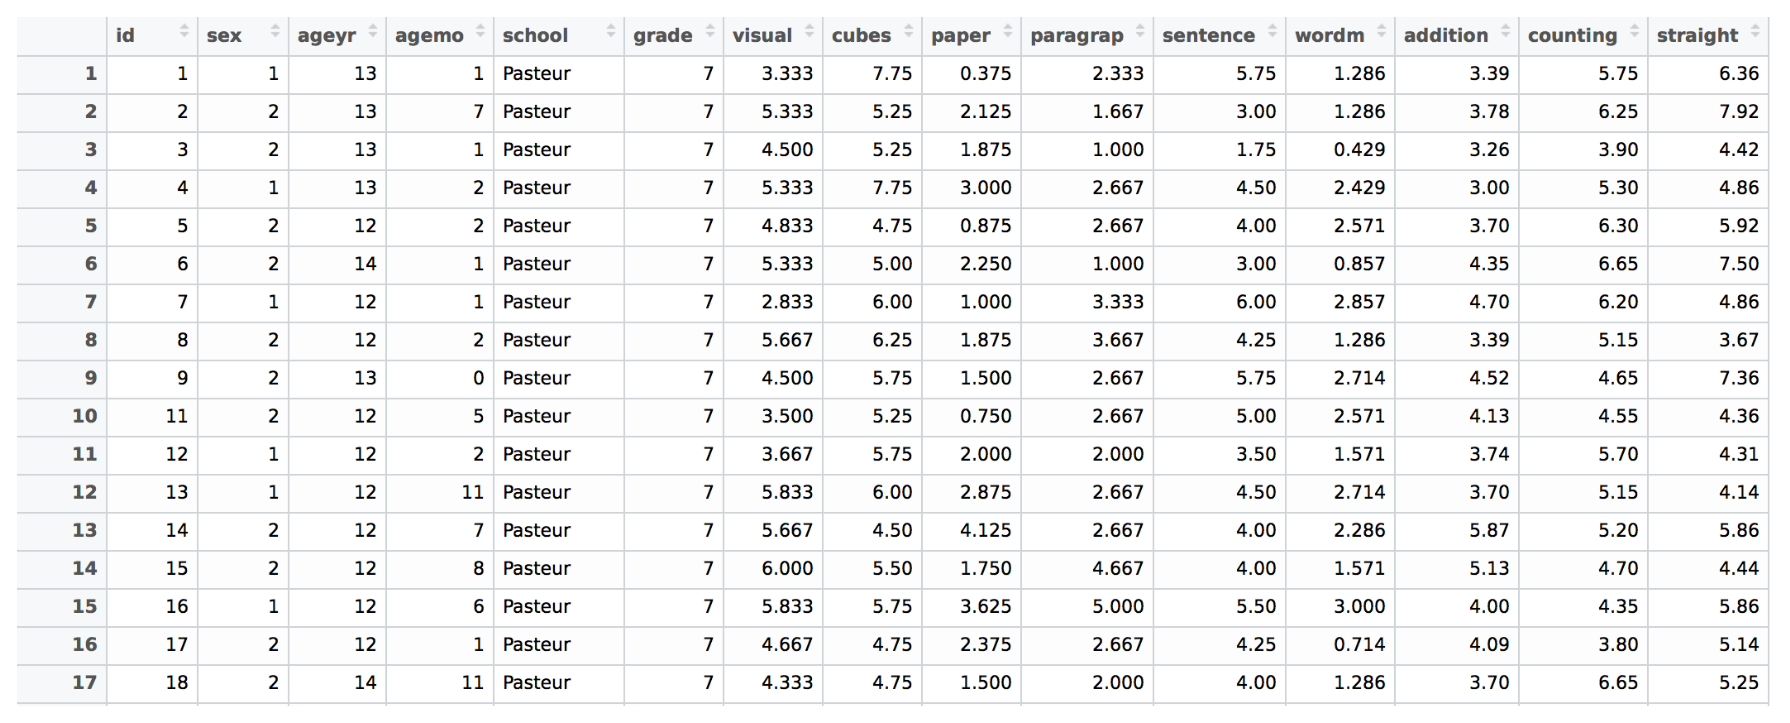
\includegraphics[width=.9\textwidth]{figs/HS.eps}}\par}


%---------------------------------------------------------------Slide-
\foilhead{Illustration}

\begin{alltt}
data(HolzingerSwineford1939, package="lavaan") 
HS <- HolzingerSwineford1939
names(HS)[7:15] <- c("\textcolor{Apricot}{visual}", "\textcolor{Apricot}{cubes}", "\textcolor{Apricot}{paper}", \hfill\textcolor{CornflowerBlue}{\ding{182}}
                     "paragrap", "sentence", "wordm", \hfill\ding{183}
                     "addition", "counting", "straight") \hfill\ding{184}
\end{alltt}

\bigskip\bigskip

{\centering \textcolor{Apricot}{visual} + \textcolor{Apricot}{cubes} +
\textcolor{Apricot}{paper} = \textcolor{CornflowerBlue}{score (composite) spatial}\par}

%---------------------------------------------------------------Slide-
\foilhead{Illustration}

Calcul des scores composites :
\begin{alltt}
HS$spatial <- rowSums(HS[,c("visual","cubes","paper")])
HS$verbal <- rowSums(HS[,c("paragrap","sentence","wordm")])
HS$speed <- rowSums(HS[,c("addition","counting","straight")])
colMeans(HS[,c("spatial","verbal","speed")])
\end{alltt}
%$

% ---------------------------------------------------------------Slide-
\foilhead{}


{\centering 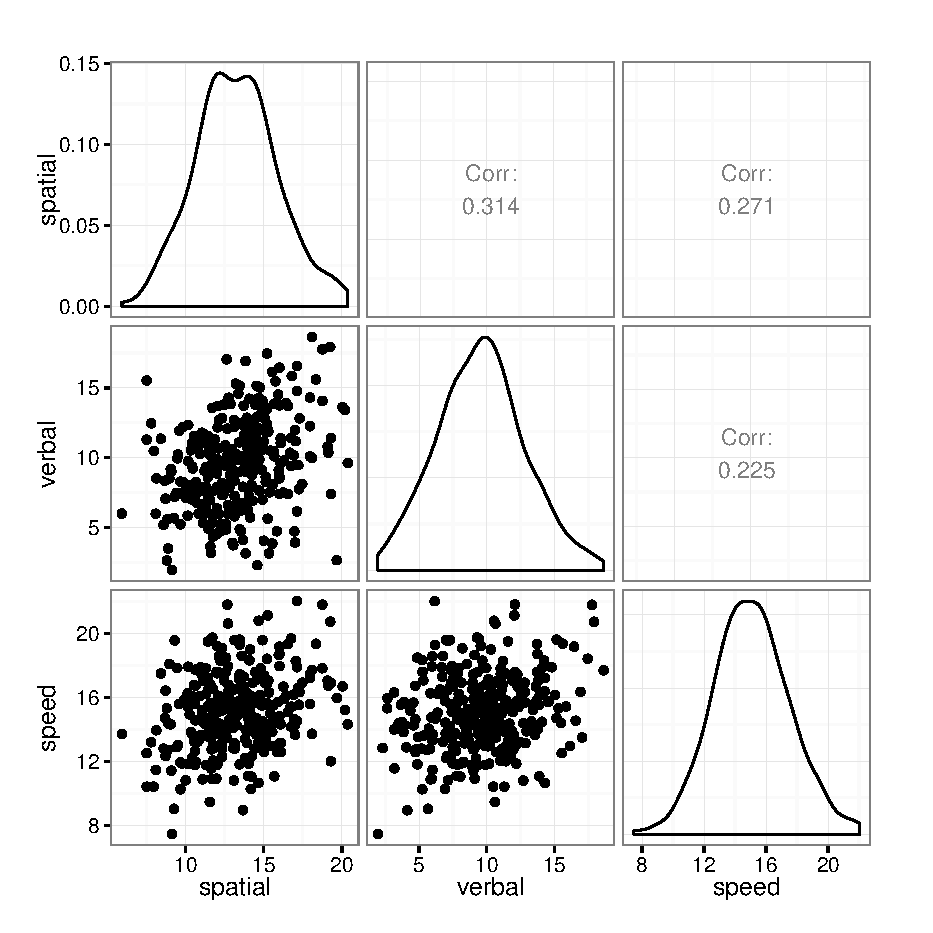
\includegraphics[width=.55\textwidth]{figs/fig-HS-ggpairs.eps}\par}

% ---------------------------------------------------------------Slide-
\foilhead{}


{\centering 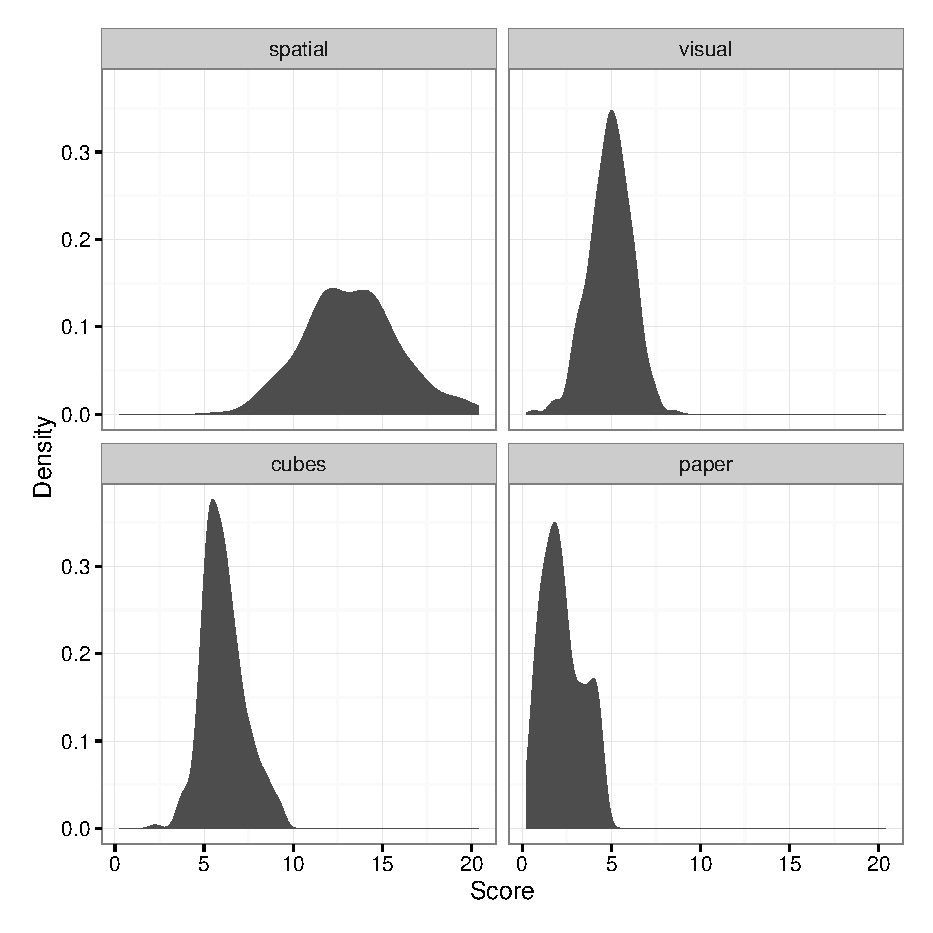
\includegraphics[width=.55\textwidth]{figs/fig-HS-hist.eps}\par}

% ---------------------------------------------------------------Slide-
\foilhead{Approche par ACP}

Les composantes $C_i$ ($i=1,\dots,p$) de l'analyse en composantes principales
(ACP) sont construites comme de simples combinaisons linéaires des $p$ variables
d'origine :
\[
C_i=\sum_{j=1}^pw_{ij}\textcolor{Apricot}{x_j}.
\]

Les charges $w_{ij}$ représentent la contribution de chaque variable dans la
composante $C_i$. Les valeurs propres représentent la part de variance expliquée
par chaque composante, et les vecteurs propres leur direction dans l'espace.

% ---------------------------------------------------------------Slide-
\foilhead{Application pour l'échelle spatiale}

\begin{alltt}
library(FactoMineR)
pca <- PCA(HS[,c("visual", "cubes", "paper")], 
           scale.unit = TRUE, graph = FALSE)  
\end{alltt}

\begin{alltt}\small
> pca$eig
       eigenvalue percentage of variance cumulative percentage of variance
comp 1  1.7221050               57.40350                          57.40350  \ding{182}
comp 2  0.7227525               24.09175                          81.49525
comp 3  0.5551425               18.50475                         100.00000  
> pca$var
$coord
           Dim.1      Dim.2      Dim.3
visual 0.7742336 -0.4082765  0.4836038  \ding{183}
cubes  0.6951525  0.7115009  0.1026133
paper  0.7996439 -0.2232247 -0.5574409

$cor
           Dim.1      Dim.2      Dim.3
visual 0.7742336 -0.4082765  0.4836038  \ding{184}
cubes  0.6951525  0.7115009  0.1026133
paper  0.7996439 -0.2232247 -0.5574409

$cos2
           Dim.1      Dim.2     Dim.3
visual 0.5994377 0.16668969 0.2338726   \ding{185}
cubes  0.4832369 0.50623355 0.0105295
paper  0.6394303 0.04982925 0.3107404
\end{alltt}
%$

Packages R pour la visualisation des résultats : \texttt{ggbiplot},
\texttt{factoextra}.

Voir aussi : \url{http://gastonsanchez.com/how-to/2012/06/17/PCA-in-R/}.

% ---------------------------------------------------------------Slide-
\foilhead{}


{\centering 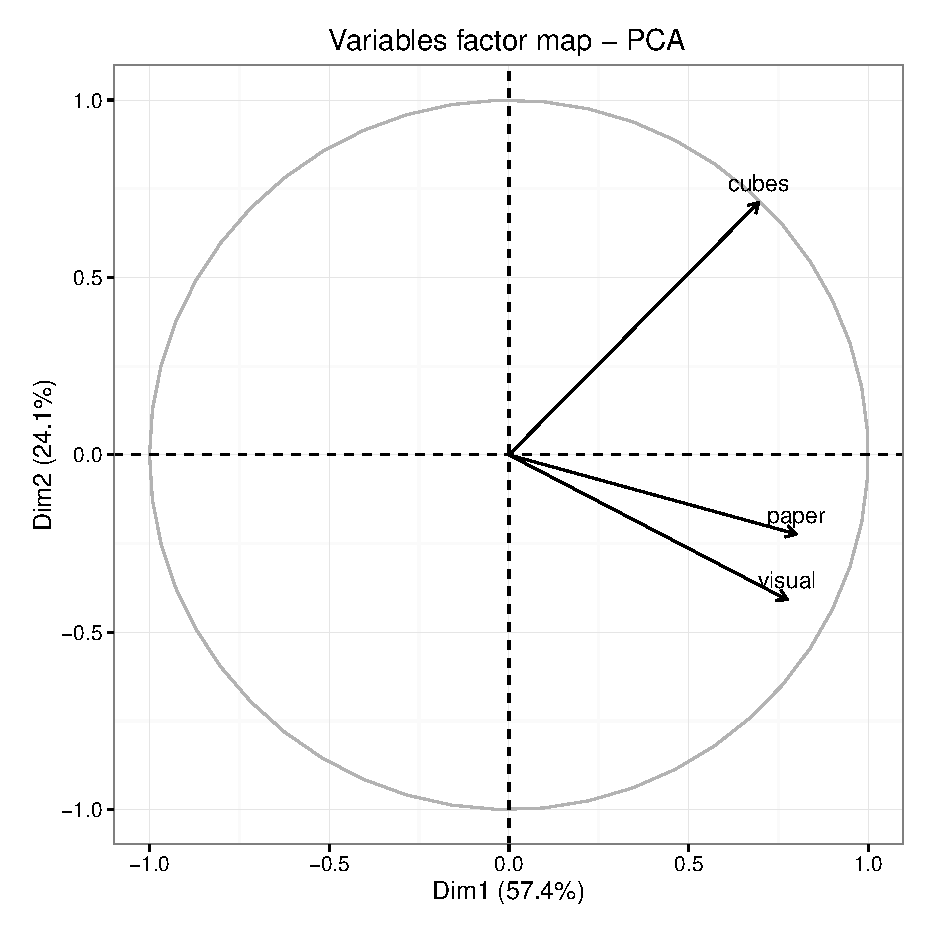
\includegraphics[width=.55\textwidth]{figs/fig-HS-pca.eps}\par}

% ---------------------------------------------------------------Slide-
\foilhead{Scores individuels}

{\centering \textcolor{Apricot}{visual} + \textcolor{Apricot}{cubes} +
\textcolor{Apricot}{paper} = \textcolor{CornflowerBlue}{score (composite) spatial}\par}

{\centering $w_{11}$\textcolor{Apricot}{visual} + $w_{12}$\textcolor{Apricot}{cubes} +
$w_{13}$\textcolor{Apricot}{paper} = PC1 $\approx$
\textcolor{CornflowerBlue}{score (factoriel) spatial}\par}

\begin{alltt}
HS$PC1 <- pca$ind$coord[,1]
cor(HS[,c("spatial","PC1")])  
\end{alltt}
%$

L'ACP peut être vue comme une méthode de réduction de dimension, de résumé
graphique d'une matrice de corrélation, voire d'inférence multivariée (sous
certaines hypothèses distributionnelles), mais dans tous les cas il suppose que
les \textcolor{Apricot}{$X_j$} sont mesurés sans erreur.

% ---------------------------------------------------------------Slide-
\foilhead{}

Fichier de données et scripts R disponibles à l'adresse suivante :\newline
{\centering \url{https://bitbucket.org/chlalanne/eespe11}\par}
\vfill

\raggedleft \scriptsize -- Typeset with \FoilTeX\ (version 2), Revision \VCRevision

\end{document}
